\documentclass[8pt]{beamer}
\usepackage[utf8]{inputenc}

\usepackage{amsmath}
\usepackage{amsfonts}
\usepackage{amssymb}
\usepackage{graphicx}
\usepackage{subfig}
\usepackage{lipsum}
\usepackage{ragged2e}
\usepackage{hyperref}
\usepackage{float}
\usepackage{url}
%\usetheme{PaloAlto}
\usepackage{amsmath,amssymb,enumerate,epsfig,bbm,calc,color,ifthen,capt-of}
\usepackage[spanish]{babel}
\usetheme{Berlin}
\usecolortheme{senac}

\newcommand{\celda}[1]{
\begin{minipage}{2.5cm}
\vspace{5mm}
#1
\vspace{5mm}
\end{minipage}
}

\author[Jhon \& Manuel]{Jhon Gesell Villanueva Portella\inst{1} \& Juan Manuel Zuñiga Mamani\inst{1}}
\title[Mecánica y Transporte de Fluidos]{Fundamentos Mecánica de Fluidos I}
\date{24 de abril de 2020} 
\subtitle{Fluido estable e inestable, flujo laminar y turbulento, fluidos compresibles e incompresibles, viscoelasticidad y viscoplasticidad}
\logo{
\includegraphics[scale=0.0375]{upch.png}}
\institute[UPCH]{
\inst{1}
Universidad Peruana Cayetano Heredia. \\Facultad de Ciencias y Filosofia. \\Escuela Profesional de Ingenieria Biomédica.\\
\vspace{2mm}

}
\AtBeginSection[]
{
\begin{frame}<beamer>{Contenido}
\tableofcontents[currentsection,currentsubsection]
\end{frame}
}


\begin{document}
\begin{frame}
\maketitle
\end{frame}
\begin{frame}{Contenido}
\tableofcontents
\end{frame}
\section{Conservación de la masa}
\begin{frame}{Flujo estable e inestable}
\justifying
Un flujo esta caracterizado por el campo de vectores de las propiedades del fluido (velocidad, presión, etc.). Si el campo de propiedades es independiente del tiempo el fluido es estable y es inestable si el campo de propiedades varía con el tiempo.

\begin{figure}[H]
\centering
\includegraphics[scale=0.2]{Section_Files/S2-imagenes-Manuel/01.png}
\end{figure}


{\tiny Biofluid Mechanics Aplications por Ali Ostadfar, pag. 19}
\end{frame}


\section{Ecuación de Navier Stokes}
\begin{frame}{Flujo Laminar y Turbulento}
\justifying
El flujo laminar y turbulento son aspectos fluídicos de un flujo viscoso. En un flujo laminar las líneas de corriente son paralelas y en el caso de una tubería circular estas son cilíndros concéntricos alrededor de la línea de flujo central.
La transición de laminar a turbulento ocurre generalmente debido a los cambios de velocidad o geometría.
\begin{figure}[H]
\centering
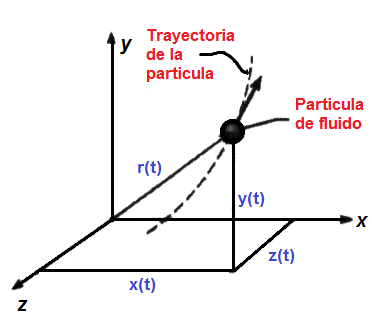
\includegraphics[scale=0.4]{Section_Files/S2-imagenes-Manuel/02.png}
\caption{Tinte sobre una corriente de flujo Newtoneano para demostrar el fluido laminar y turbulento.}
\end{figure}
{\tiny Biofluid Mechanics Aplications por Ali Ostadfar, pag. 20}
\end{frame}

\begin{frame}{Perfil de velocidad}
\justifying
Es un diagrama de vectores de velocidad de una corriente de fluido como una función de la distancia perpendicular a la dirección del flujo.
\begin{figure}[H]
\centering
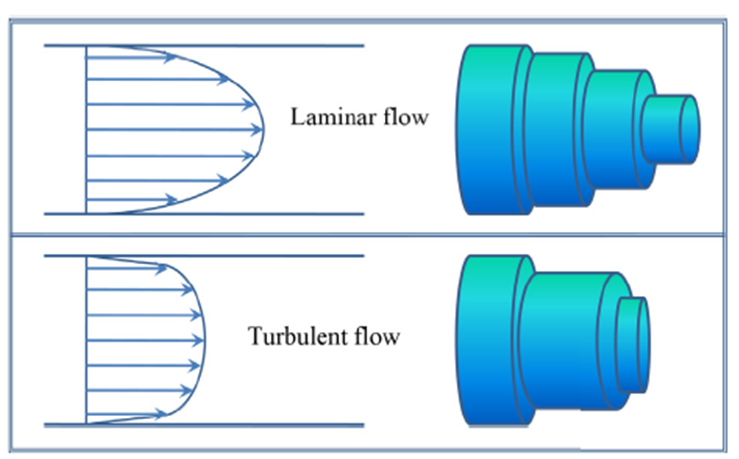
\includegraphics[scale=0.4]{Section_Files/S2-imagenes-Manuel/03.png}
\caption{Esquema de perfil de velocidad para un flujo laminar y turbulento.}
\end{figure}
{\tiny Biofluid Mechanics Aplications por Ali Ostadfar, pag. 20}
\end{frame}

\begin{frame}{Flujo laminar}
\justifying
Para un flujo viscoso a través de un canal circular, el perfil de velocidad axial esta dado por:
\begin{figure}[H]
\centering
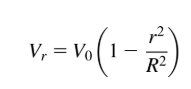
\includegraphics[scale=0.4]{Section_Files/S2-imagenes-Manuel/04.png}
\end{figure}
\begin{figure}[H]
\centering
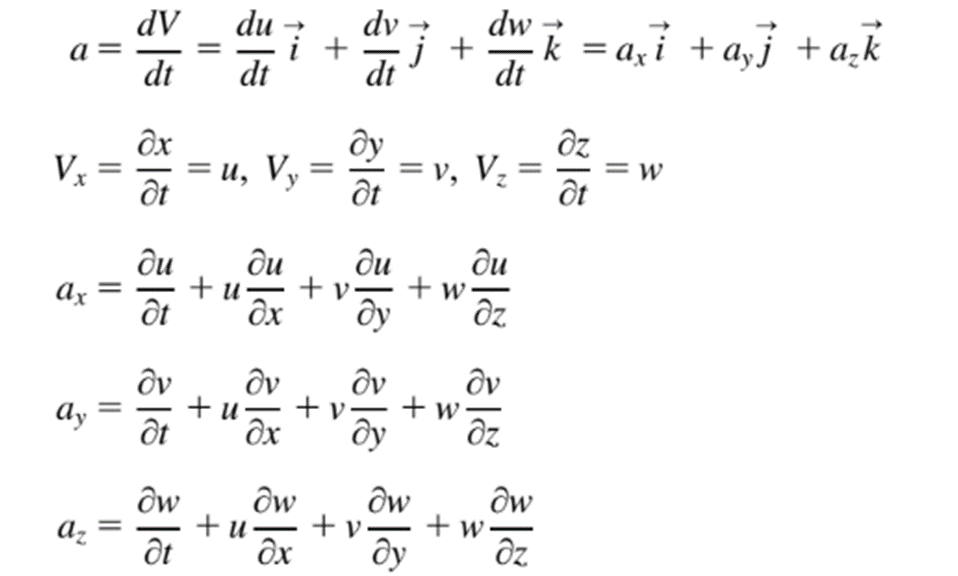
\includegraphics[scale=0.3]{Section_Files/S2-imagenes-Manuel/05.png}
\end{figure}
{\tiny Biofluid Mechanics Aplications por Ali Ostadfar, pag. 21}
\end{frame}

\begin{frame}{Flujo turbulento}
\justifying
\begin{itemize}
\item El flujo varía constantemente y este tiene un comportamiento caótico.
\item El esfuerzo cortante entre capas aumenta.
\item El número de Reynolds ayuda a evaluar si el fluido es laminar o turbulento.
\end{itemize}

\begin{figure}[H]
\centering
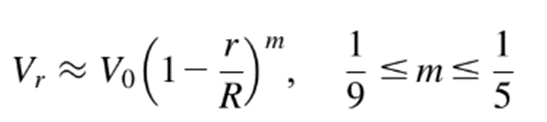
\includegraphics[scale=0.25]{Section_Files/S2-imagenes-Manuel/06.png}
\caption{Where Vr is axial velocity as a function of radius. Vo is maximun velocity at the certerline, r is radial distance from the centerline and R is radius of the channel.}
\end{figure}
\begin{figure}[H]
\centering
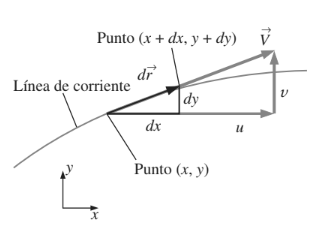
\includegraphics[scale=0.3]{Section_Files/S2-imagenes-Manuel/08.png}
\end{figure}
{\tiny Biofluid Mechanics Aplications por Ali Ostadfar, pag. 21}
\end{frame}

\begin{frame}{Flujo turbulento - Ejercicio}
\justifying
\begin{figure}[H]
\centering
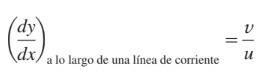
\includegraphics[scale=0.4]{Section_Files/S2-imagenes-Manuel/09.png}
\end{figure}
{\tiny Biofluid Mechanics Aplications por Ali Ostadfar, pag. 31}
\end{frame}

\begin{frame}{Flujo turbulento - Ejercicio}
\justifying
\begin{figure}[H]
\centering
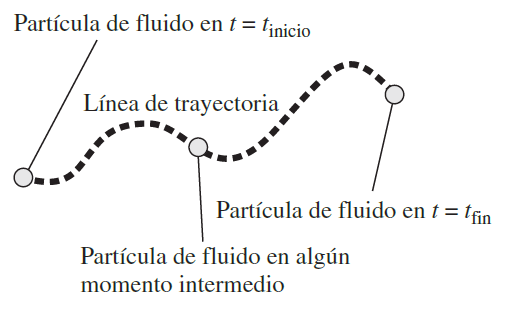
\includegraphics[scale=0.4]{Section_Files/S2-imagenes-Manuel/10.png}
\end{figure}
{\tiny Biofluid Mechanics Aplications por Ali Ostadfar, pag. 31}
\end{frame}

\begin{frame}{Flujo turbulento - Ejercicio}
\justifying
\begin{figure}[H]
\centering
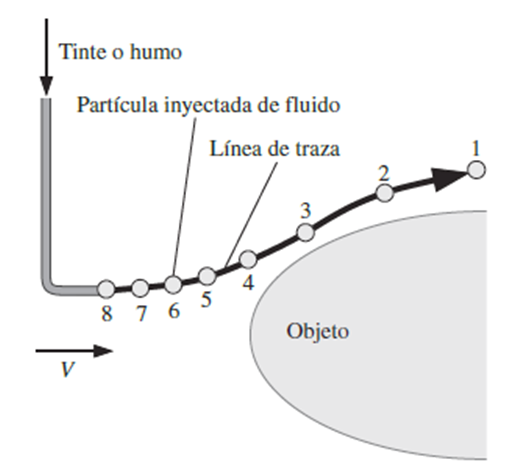
\includegraphics[scale=0.4]{Section_Files/S2-imagenes-Manuel/11.png}
\end{figure}
{\tiny Biofluid Mechanics Aplications por Ali Ostadfar, pag. 32}
\end{frame}

\begin{frame}{Flujo turbulento - Ejercicio}
\justifying
\begin{figure}[H]
\centering
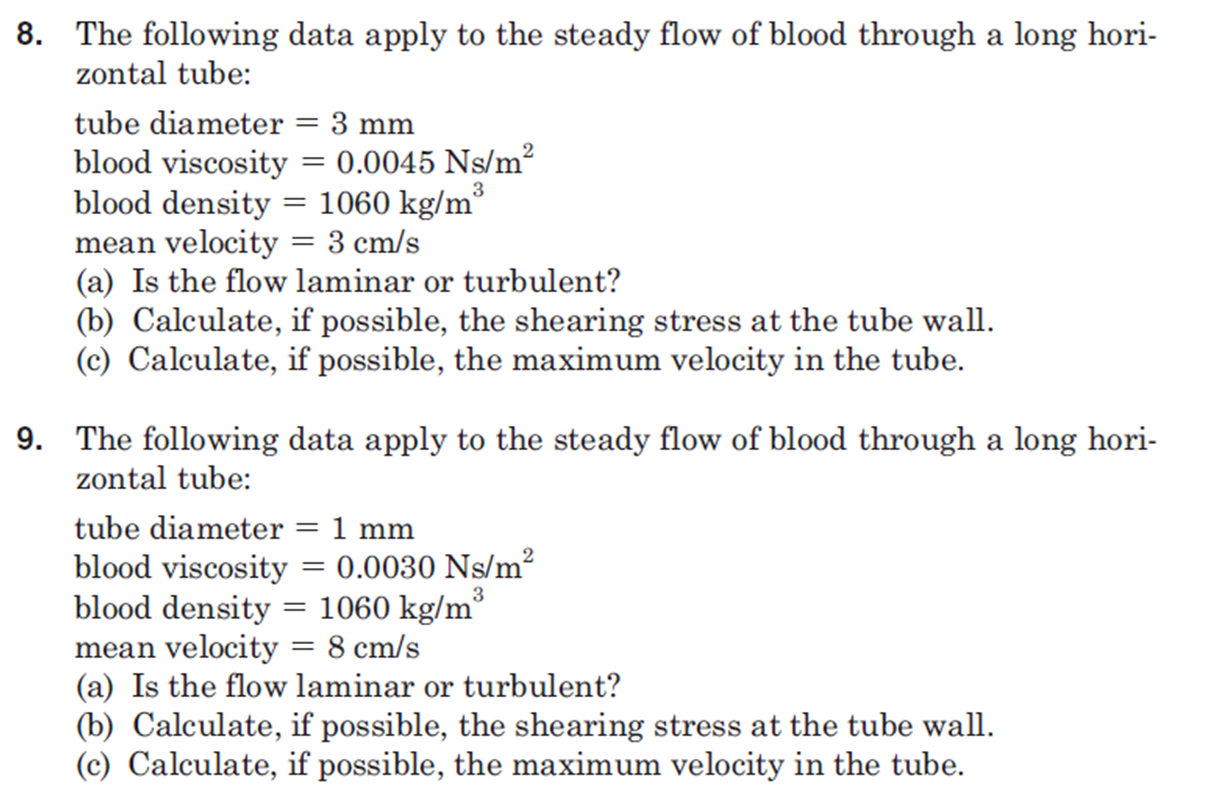
\includegraphics[scale=0.4]{Section_Files/S2-imagenes-Manuel/12.png}
\end{figure}
{\tiny Biofluid Mechanics Aplications por Ali Ostadfar, pag. 32}
\end{frame}

\begin{frame}{Condiciones de borde y no deslizamiento}
\justifying
Las ecuaciones tienen un rol importante en las aplicaciones físicas. Las ecuaciones que gobiernan las características físicas, como presión y velocidad, están definidas por ecuaciones diferenciales parciales. Para calcular estas ecuaciones es necesario conocer datos iniciales, como el camp'o de velocidades en el campo de los fluidos. Estos datos son conocidos como condiciones de contorno o borde.
\begin{figure}[H]
\centering
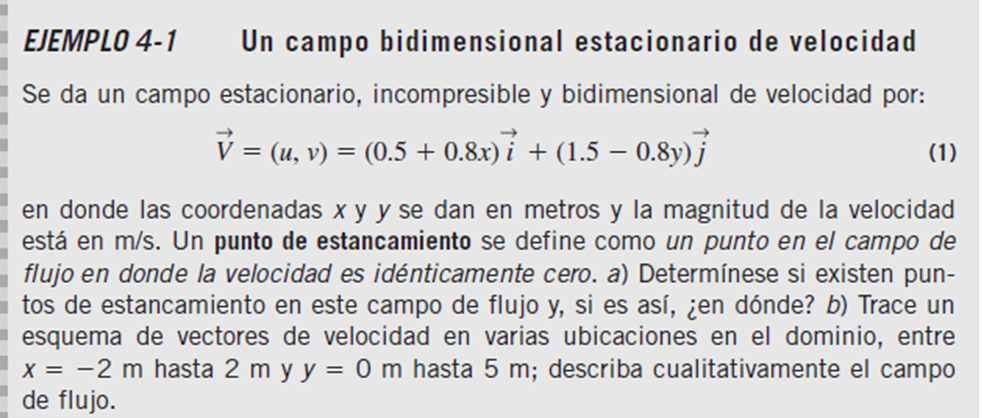
\includegraphics[scale=0.4]{Section_Files/S2-imagenes-Manuel/13.png}
\caption{Esquema de condición de contorno de no deslizamiento. La velocidad tangencial en el punto entre la interface líquido-sólido de la pared de la tubería es igual a cero ($V(R)=0m/s)$.}
\end{figure}
{\tiny Biofluid Mechanics Aplications por Ali Ostadfar, pag. 32}
\end{frame}
\section{Ecuación de Bernoulli}
\begin{frame}{Flujo estable e inestable}
\justifying
Texto


{\tiny Libro}
\end{frame}
\section{Ecuación de Hagen}
\begin{frame}{Flujo estable e inestable}
\justifying
Texto


{\tiny Libro}
\end{frame}
\section{Refuerzo}
%\subsection{Teórico}
\begin{frame}{Turbulencia}
\justifying
La más difundida forma reflujo de fluido en la naturaleza es una forma irregular y caótica.
Si un flujo irregular caótico también es difuso y disipativo, entonces se dice que el movimiento de fluido forma un campo de flujo turbulento. La evaluación y computación de los campos de flujo turbulento por medio de los métodos deterministas, los cuales en principio se aplican para resolver los más pequeños detalles de un campo, es un trabajo extgremadamente agotador y aburrida y al mismo tiempo demasiado detallado para objetivos de ingeniero. Así para anlizar los campos de flujo turbulento hay que usar métodos estadísticos apropiados.\\
{\tiny Introducción a la dinámica de fluidos por Yuri N. Skiba, pag. 377}
\end{frame}

\begin{frame}{Flujos turbulentos - 01/03}
\justifying
Un flujo viscoso puede ser clasificado como flujo laminar o flujo turbulento. En un flujoi laminar el fluido fluye sin mezclado significativo de sus partículas próximas entre sí. Si se inyectara un colorante, el flujo no se mezclaría con el fluido cercano excepto por actividad molecular; conservará su identidad durante un lapto se tiempo relativamente largo. Los esfuerzos cortantes viscosos siempre influyen en un flujo laminar.

En un flujo turbulento los movimientos del fluido varían irregularmente de tal suerte que las cantidades tales como velocidad y presión muestran una variación aleatoria con el tiempo y las coordenadas espaciales. Las cantidades físicas con frecuencia se describen mediante promedios estadísticos (Chorin, 1994). Un colorante inyectado en un fluijo turbulento se mezclará de inmediato por la acción del movomiento aleatorio de sus partículas; rápidamente perderá su identidad en este proceso de difusión.\\
{\tiny Introducción a la dinámica de fluidos por Yuri N. Skiba, pag. 377}
\end{frame}

\begin{frame}{Flujos turbulentos - 02/03}
\justifying
Un flujo laminar y un flujo turbulento pueden ser observados mediante la realización de un experimento simple con una llave de agua. Si abrimos la llave un poco entonces el agua fluye lentamente como una corriente silenciosa. Este es un flujo laminar. Y si continuamos abriendo más la llave se puede observar cómo el flujo se vuelve turbulento. Note que un flujo turbulento se desarrolla con un gasto relativamente pequeño.

En aplicaciones prácticas a menudo se estudian el desarrollo de flujos turbulentos en un tubo (Cengel y Cimbala, 2006). Aun cuando en condiciones de laboratorio cuidadosamente controladas, se han observado flujos laminares con números de Reynolds hasta de 400000 en flujos turbulentos desarrollados en tubos, se supone que los flujos turbulentos ocurren en tubos en condiciones de operación estándar siempre que el número de Reynolds exceda de 4000; entre 2000 y 4000 se supone que el flujo oscila de una manera aleatoria entre laminar y turbulento.\\
{\tiny Introducción a la dinámica de fluidos por Yuri N. Skiba, pag. 378}
\end{frame}

\begin{frame}{Flujos turbulentos - 03/03}
\justifying
\begin{figure}[H]
\centering
\includegraphics[scale=0.4]{Section_Files/S2-imagenes-Jhon/Book-IMF/01.png}
\caption{Bosquejos de (a) flujo laminar en un tubo indicado por una vena de tinta;
(b) transición a un flujo turbulento; (c) transición a un flujo turbulento como se ve cuando está iluminada por un resplandor (Reynolds, 1883).}
\end{figure}
{\tiny Introducción a la dinámica de fluidos por Yuri N. Skiba, pag. 378}
\end{frame}

\begin{frame}{Flujos turbulentos - 03/03}
\justifying
Considere, por ejemplo, agua a 20  $^{\circ}$C fluyente en un tubo de 5mm de diámetro; se requiere sólo una velocidad media de 0.8 m/s para que el flujo sea turbulento. Ésta es la situación siempre que se bebe agua de un bebedero. Con tubos de mayor diámetro la velocidad media es suficientemente grande así que en la mayoría de las situaciones de ingeniería se producen un flujo turbulento. El perfil de velocidad en un flujo en tubería totalmente desarrollado es parabólico en el flujo lamniar, pero es mucho más plano en el flujo turbulento. Además, los gradientes de velocidad en la pared son mayores para flujo turbulento que para flujo laminar, aun cuando la capa límite turbulenta sea más grande gruesa que la capa laminar para ael mismo valor de velocidad de flujo libre.

Ninguna definición corta pero bastante completa de la turbulencia parece ser posible (Frisch, 1995). Uno puede formular un breve resumen, más bien que una definición formal. Quizás el mejor es que la turbulencia es un estado de inestabilidad continuar. Cada vez que un flujo se cambia a consecuencia de una inestabilidad, capacidad de predecir los detalles del movimiento son reducidos. Cuando las inestabilidades sucesivas han reducido el nivel de predicción tanto que es apropiado describir un flujo estadísticamente, más bien que en cada detalle, entonces se dice que el flujo es turbulento.
{\tiny Introducción a la dinámica de fluidos por Yuri N. Skiba, pag. 379}
\end{frame}

\begin{frame}{Flujos turbulentos - 03/03}
\justifying
\begin{figure}[H]
\centering
\includegraphics[scale=0.4]{Section_Files/S2-imagenes-Jhon/Book-IMF/01.png}
\caption{Bosquejos de (a) flujo laminar en un tubo indicado por una vena de tinta;
(b) transición a un flujo turbulento; (c) transición a un flujo turbulento como se ve cuando está iluminada por un resplandor (Reynolds, 1883).}
\end{figure}
{\tiny Introducción a la dinámica de fluidos por Yuri N. Skiba, pag. 378}
\end{frame}

% Victor Streeter - Mecánica de Fluidos

\begin{frame}{Flujo viscoso: tuberías y canales}
\justifying
Fluidos reales en situaciones en las cuales las irreversibilidades son importantes. La viscosidad es la propiedad del fluido que causa los esfuerzos cortantes en fluidos en movimiento. La viscosidad tamibén es uno de los medios mediante el cual se desarrollan pérdidas. En flujos turbulentos, los movimientos aleatorios de fluidos superpuestos al promedio, crean esfuerzos cortantes en fluidos en movimiento. La viscosidad también es uno de los medios mediante el cual se desarrollan pérdidas. En flujos turbulentos, los movimientos aleatorios de fluidos superpuestos al promedio, crean esfuerzos cortantes aparentes que son más importantes que en aquellos debido a los esfuerzos cortantes viscosos.
{\tiny Mecánica de fluidos por Victor Streeter, pág. 259}
\end{frame}

\begin{frame}{Flujos laminares y turbulentos: FLujos internos y externos}
\justifying
El número de Reynolds:
El flujo laminar se defime como el flujo en el cual el fluido se mueve en capas, o láminas, que se deslizan suavemente una sobre otra adyacente, únicamente con intercambio molecular de momentum. Cualquier tendencia a la inestabilidad y turbulencia son atenuadas por las fuerzas cortantes viscosas que resisten el movimineot relativo de capas fluidas adyacentes. Sin embargo, en el flujo turbulento las partículas fluidas tienen un movimiento muy errático, con un intercambio de momentum transfersal violento. La naturaleza del flujo, es decir, si es laminar o turbulento, y su posición relativa en una escala que muestra la importancia relativa de las tendencias turbulentas a laminares están indicadas por el número de Reynolds.
{\tiny Mecánica de fluidos por Victor Streeter, pág. 260}
\end{frame}

\begin{frame}{Flujos laminares y turbulentos: FLujos internos y externos}
\justifying
Se dice que dos casos de flujo son dinámicamente similares cuando:
\begin{itemize}
\item Éstos son geométricamente similares, es decir, que las dimensiones lineales correspondientes tienen una relación constante.
\item Los correspondientes polígonos de fuerza son geométricamente similares, o que las presiones en puntos correspondientes tienen una relación constante.
\end{itemize}
Al considerar dos situaciones de flujo geométricamente similares, Reynolds dedujo que éstos serían dinámicamente simialres si las ecuaciones diferenciales generales que describían sus flujos fueran idénticas. Al cambiar las unidades de masa, longitud y tiempo en un cambio de ecuaciones y al determinar la condición que debe ser satisfecha para hacerlas idénticas a las ecuaciones originales, Reynolds encontró que el grupo adimensional 
{\tiny Mecánica de fluidos por Victor Streeter, pág. 260}
\end{frame}

% PROBLEMAS RESUELTOS POR JOSEP BERGADÁ

%% PROBLEMAS RESUELTOS: Propiedades de fluidos
%\subsection{Ejercicios}
\begin{frame}{PROBLEMAS RESUELTOS: Propiedades de fluidos - 01/12}
\justifying
Problema 01:
\begin{figure}[H]
\centering
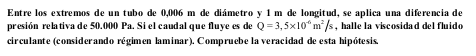
\includegraphics[scale=0.6]{Section_Files/S2-imagenes-Jhon/Book-ProbResuelts/P01-E01.png}
\end{figure}
{\tiny Mecánica de fluidos - Problemas resueltos por Josep Bergada Graño, pág. 001}
\end{frame}

\begin{frame}{PROBLEMAS RESUELTOS: Propiedades de fluidos - 02/12}
\justifying
Solución:
\begin{figure}[H]
\centering
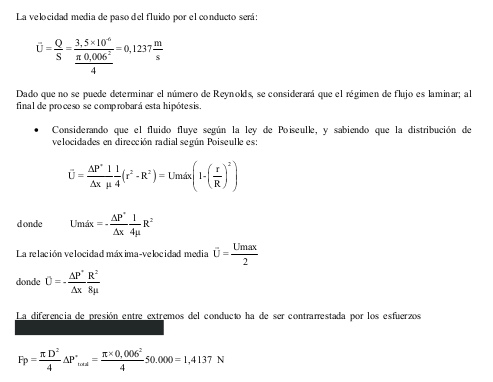
\includegraphics[scale=0.4]{Section_Files/S2-imagenes-Jhon/Book-ProbResuelts/P01-E02.png}
\end{figure}
Continúa...\\
{\tiny Mecánica de fluidos - Problemas resueltos por Josep Bergada Graño, pág. 001}
\end{frame}

\begin{frame}{PROBLEMAS RESUELTOS: Propiedades de fluidos - 03/12}
\justifying
\begin{figure}[H]
\centering
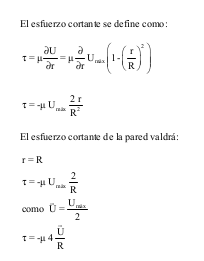
\includegraphics[scale=0.4]{Section_Files/S2-imagenes-Jhon/Book-ProbResuelts/P01-E03.png}
\end{figure}
Continúa...\\
{\tiny Mecánica de fluidos - Problemas resueltos por Josep Bergada Graño, pág. 002}
\end{frame}

\begin{frame}{PROBLEMAS RESUELTOS: Propiedades de fluidos - 04/12}
\justifying
\begin{figure}[H]
\centering
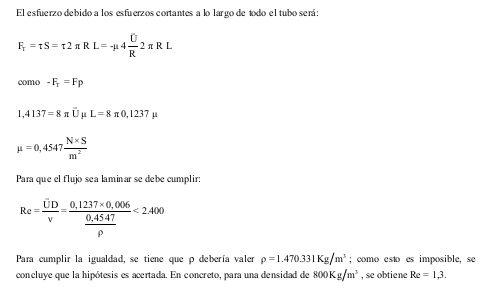
\includegraphics[scale=0.4]{Section_Files/S2-imagenes-Jhon/Book-ProbResuelts/P01-E04.png}
\end{figure}
{\tiny Mecánica de fluidos - Problemas resueltos por Josep Bergada Graño, pág. 002}
\end{frame}

\begin{frame}{PROBLEMAS RESUELTOS: Propiedades de fluidos - 05/12}
\justifying
Problema 02:
\begin{figure}[H]
\centering
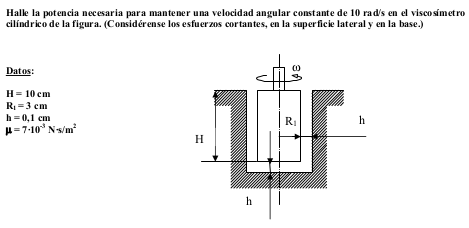
\includegraphics[scale=0.4]{Section_Files/S2-imagenes-Jhon/Book-ProbResuelts/P02-E01.png}
\end{figure}
{\tiny Mecánica de fluidos - Problemas resueltos por Josep Bergada Graño, pág. 003}
\end{frame}

\begin{frame}{PROBLEMAS RESUELTOS: Propiedades de fluidos - 06/12}
\justifying
Solución:
\begin{figure}[H]
\centering
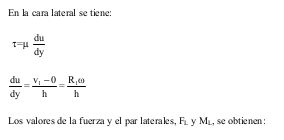
\includegraphics[scale=0.4]{Section_Files/S2-imagenes-Jhon/Book-ProbResuelts/P02-E02.png}
\end{figure}
Continúa...\\
{\tiny Mecánica de fluidos - Problemas resueltos por Josep Bergada Graño, pág. 003}
\end{frame}

\begin{frame}{PROBLEMAS RESUELTOS: Propiedades de fluidos - 07/12}
\justifying
\begin{figure}[H]
\centering
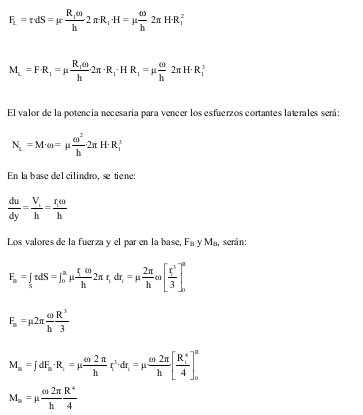
\includegraphics[scale=0.4]{Section_Files/S2-imagenes-Jhon/Book-ProbResuelts/P02-E03.png}
\end{figure}
Continúa...\\
{\tiny Mecánica de fluidos - Problemas resueltos por Josep Bergada Graño, pág. 004}
\end{frame}

\begin{frame}{PROBLEMAS RESUELTOS: Propiedades de fluidos - 08/12}
\justifying
\begin{figure}[H]
\centering
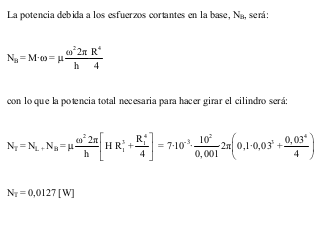
\includegraphics[scale=0.4]{Section_Files/S2-imagenes-Jhon/Book-ProbResuelts/P02-E04.png}
\end{figure}
{\tiny Mecánica de fluidos - Problemas resueltos por Josep Bergada Graño, pág. 004}
\end{frame}

\begin{frame}{PROBLEMAS RESUELTOS: Propiedades de fluidos - 09/12}
\justifying
Problema 03:
\begin{figure}[H]
\centering
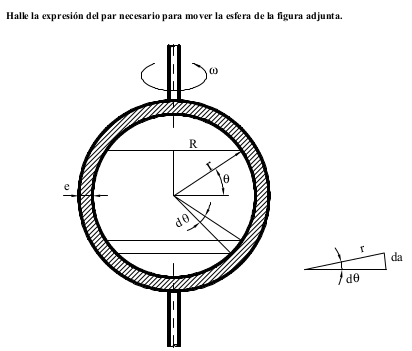
\includegraphics[scale=0.4]{Section_Files/S2-imagenes-Jhon/Book-ProbResuelts/P03-E01.png}
\end{figure}
{\tiny Mecánica de fluidos - Problemas resueltos por Josep Bergada Graño, pág. 005}
\end{frame}

\begin{frame}{PROBLEMAS RESUELTOS: Propiedades de fluidos - 10/12}
\justifying
Solución:
\begin{figure}[H]
\centering
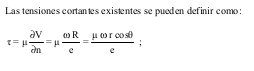
\includegraphics[scale=0.6]{Section_Files/S2-imagenes-Jhon/Book-ProbResuelts/P03-E02.png}
\end{figure}
Continúa...\\
{\tiny Mecánica de fluidos - Problemas resueltos por Josep Bergada Graño, pág. 005}
\end{frame}

\begin{frame}{PROBLEMAS RESUELTOS: Propiedades de fluidos - 11/12}
\justifying
\begin{figure}[H]
\centering
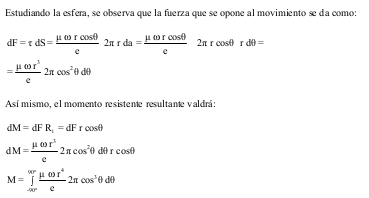
\includegraphics[scale=0.6]{Section_Files/S2-imagenes-Jhon/Book-ProbResuelts/P03-E03.png}
\end{figure}
Continúa...\\
{\tiny Mecánica de fluidos - Problemas resueltos por Josep Bergada Graño, pág. 006}
\end{frame}

\begin{frame}{PROBLEMAS RESUELTOS: Propiedades de fluidos - 12/12}
\justifying
\begin{figure}[H]
\centering
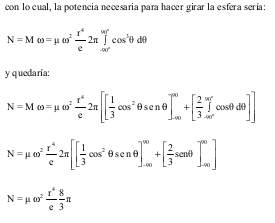
\includegraphics[scale=0.6]{Section_Files/S2-imagenes-Jhon/Book-ProbResuelts/P03-E04.png}
\end{figure}
{\tiny Mecánica de fluidos - Problemas resueltos por Josep Bergada Graño, pág. 006}
\end{frame}

%% PROBLEMAS RESUELTOS: Flujo con viscosidad dominante

\begin{frame}{PROBLEMAS RESUELTOS: Flujo con viscosidad dominante - 01/20}
\justifying
Problema 04:
\begin{figure}[H]
\centering
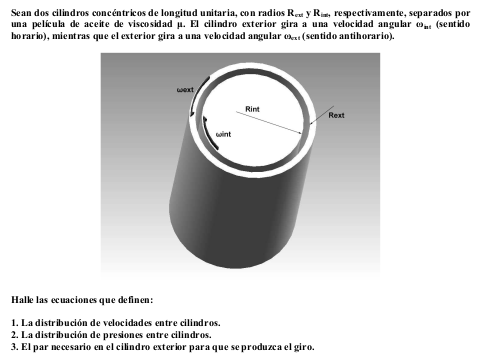
\includegraphics[scale=0.4]{Section_Files/S2-imagenes-Jhon/Book-ProbResuelts/P35-E01.png}
\end{figure}
{\tiny Mecánica de fluidos - Problemas resueltos por Josep Bergada Graño, pág. 127}
\end{frame}

\begin{frame}{PROBLEMAS RESUELTOS: Flujo con viscosidad dominante - 02/20}
\justifying
Solución:
\begin{figure}[H]
\centering
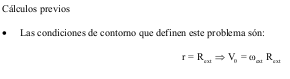
\includegraphics[scale=0.5]{Section_Files/S2-imagenes-Jhon/Book-ProbResuelts/P35-E02.png}
\end{figure}
Continúa...\\
{\tiny Mecánica de fluidos - Problemas resueltos por Josep Bergada Graño, pág. 127}
\end{frame}

\begin{frame}{PROBLEMAS RESUELTOS: Flujo con viscosidad dominante - 03/20}
\justifying
\begin{figure}[H]
\centering
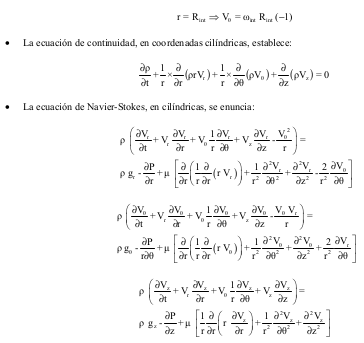
\includegraphics[scale=0.5]{Section_Files/S2-imagenes-Jhon/Book-ProbResuelts/P35-E03.png}
\end{figure}
Continúa...\\
{\tiny Mecánica de fluidos - Problemas resueltos por Josep Bergada Graño, pág. 128}
\end{frame}

\begin{frame}{PROBLEMAS RESUELTOS: Flujo con viscosidad dominante - 04/20}
\justifying
\begin{figure}[H]
\centering
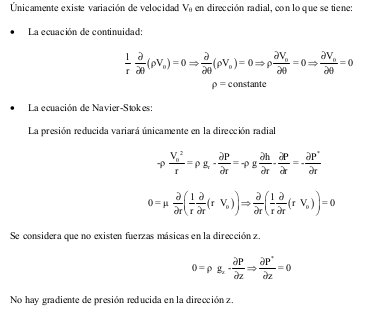
\includegraphics[scale=0.5]{Section_Files/S2-imagenes-Jhon/Book-ProbResuelts/P35-E04.png}
\end{figure}
Continúa...\\
{\tiny Mecánica de fluidos - Problemas resueltos por Josep Bergada Graño, pág. 128}
\end{frame}

\begin{frame}{PROBLEMAS RESUELTOS: Flujo con viscosidad dominante - 05/20}
\justifying
\begin{figure}[H]
\centering
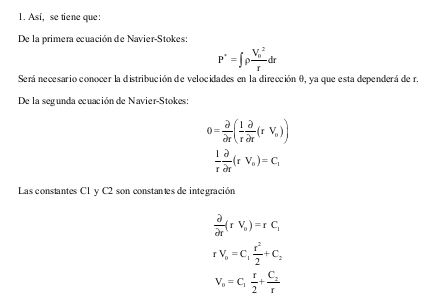
\includegraphics[scale=0.5]{Section_Files/S2-imagenes-Jhon/Book-ProbResuelts/P35-E05.png}
\end{figure}
Continúa...\\
{\tiny Mecánica de fluidos - Problemas resueltos por Josep Bergada Graño, pág. 129}
\end{frame}

\begin{frame}{PROBLEMAS RESUELTOS: Flujo con viscosidad dominante - 06/20}
\justifying
\begin{figure}[H]
\centering
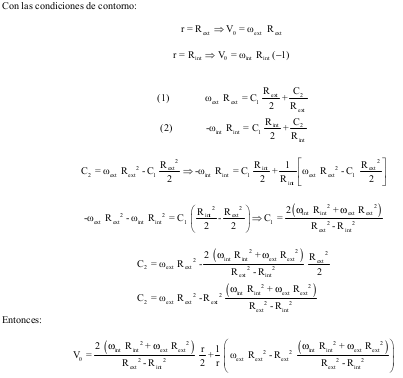
\includegraphics[scale=0.4]{Section_Files/S2-imagenes-Jhon/Book-ProbResuelts/P35-E06.png}
\end{figure}
Continúa...\\
{\tiny Mecánica de fluidos - Problemas resueltos por Josep Bergada Graño, pág. 129}
\end{frame}

\begin{frame}{PROBLEMAS RESUELTOS: Flujo con viscosidad dominante - 07/20}
\justifying
\begin{figure}[H]
\centering
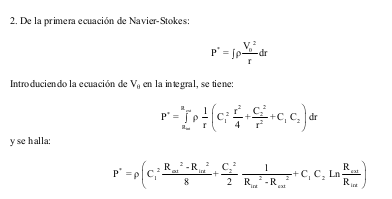
\includegraphics[scale=0.5]{Section_Files/S2-imagenes-Jhon/Book-ProbResuelts/P35-E07.png}
\end{figure}
Continúa...\\
{\tiny Mecánica de fluidos - Problemas resueltos por Josep Bergada Graño, pág. 130}
\end{frame}

\begin{frame}{PROBLEMAS RESUELTOS: Flujo con viscosidad dominante - 08/20}
\justifying
\begin{figure}[H]
\centering
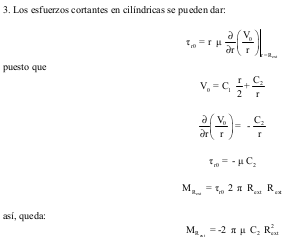
\includegraphics[scale=0.5]{Section_Files/S2-imagenes-Jhon/Book-ProbResuelts/P35-E08.png}
\end{figure}
{\tiny Mecánica de fluidos - Problemas resueltos por Josep Bergada Graño, pág. 130}
\end{frame}

\begin{frame}{PROBLEMAS RESUELTOS: Flujo con viscosidad dominante - 09/20}
\justifying
\begin{figure}[H]
\centering
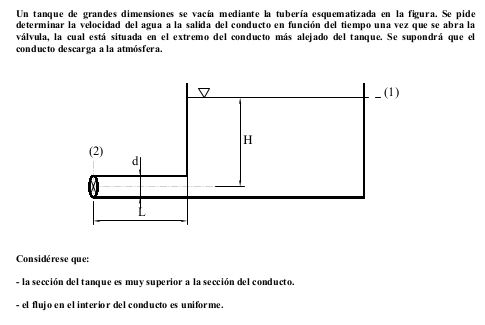
\includegraphics[scale=0.5]{Section_Files/S2-imagenes-Jhon/Book-ProbResuelts/P38-E01.png}
\end{figure}
{\tiny Mecánica de fluidos - Problemas resueltos por Josep Bergada Graño, pág. 141}
\end{frame}

\begin{frame}{PROBLEMAS RESUELTOS: Flujo con viscosidad dominante - 10/20}
\justifying
Solución:
\begin{figure}[H]
\centering
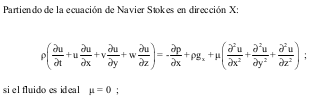
\includegraphics[scale=0.5]{Section_Files/S2-imagenes-Jhon/Book-ProbResuelts/P38-E02.png}
\end{figure}
Continúa...\\
{\tiny Mecánica de fluidos - Problemas resueltos por Josep Bergada Graño, pág. 141}
\end{frame}

\begin{frame}{PROBLEMAS RESUELTOS: Flujo con viscosidad dominante - 09/20}
\justifying
\begin{figure}[H]
\centering
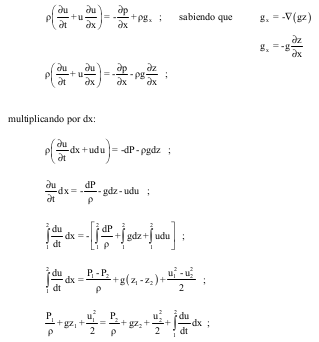
\includegraphics[scale=0.5]{Section_Files/S2-imagenes-Jhon/Book-ProbResuelts/P38-E03.png}
\end{figure}
Continúa...\\
{\tiny Mecánica de fluidos - Problemas resueltos por Josep Bergada Graño, pág. 142}
\end{frame}

\begin{frame}{PROBLEMAS RESUELTOS: Flujo con viscosidad dominante - 09/20}
\justifying
\begin{figure}[H]
\centering
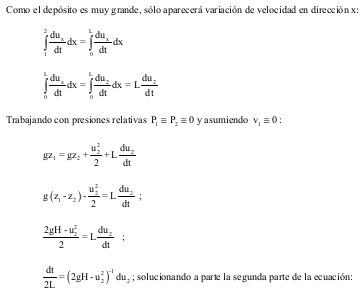
\includegraphics[scale=0.5]{Section_Files/S2-imagenes-Jhon/Book-ProbResuelts/P38-E04.png}
\end{figure}
Continúa...\\
{\tiny Mecánica de fluidos - Problemas resueltos por Josep Bergada Graño, pág. 142}
\end{frame}

\begin{frame}{PROBLEMAS RESUELTOS: Flujo con viscosidad dominante - 10/20}
\justifying
\begin{figure}[H]
\centering
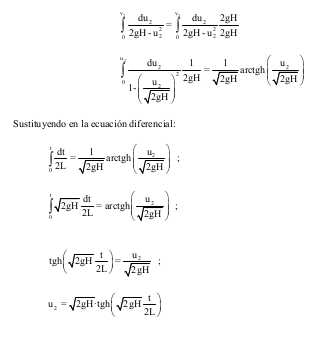
\includegraphics[scale=0.5]{Section_Files/S2-imagenes-Jhon/Book-ProbResuelts/P38-E05.png}
\end{figure}
{\tiny Mecánica de fluidos - Problemas resueltos por Josep Bergada Graño, pág. 143}
\end{frame}

\begin{frame}{PROBLEMAS RESUELTOS: Flujo con viscosidad dominante - 11/20}
\justifying
Problema 05:
\begin{figure}[H]
\centering
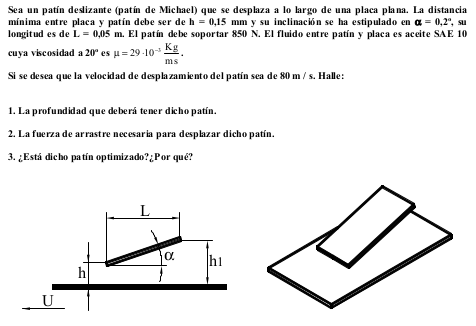
\includegraphics[scale=0.5]{Section_Files/S2-imagenes-Jhon/Book-ProbResuelts/P40-E01.png}
\end{figure}
{\tiny Mecánica de fluidos - Problemas resueltos por Josep Bergada Graño, pág. 149}
\end{frame}

\begin{frame}{PROBLEMAS RESUELTOS: Flujo con viscosidad dominante - 12/20}
\justifying
Solución:
\begin{figure}[H]
\centering
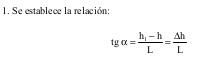
\includegraphics[scale=0.5]{Section_Files/S2-imagenes-Jhon/Book-ProbResuelts/P40-E02.png}
\end{figure}
Continúa...\\
{\tiny Mecánica de fluidos - Problemas resueltos por Josep Bergada Graño, pág. 149}
\end{frame}

\begin{frame}{PROBLEMAS RESUELTOS: Flujo con viscosidad dominante - 13/20}
\justifying
\begin{figure}[H]
\centering
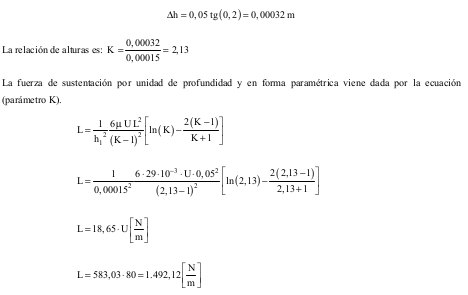
\includegraphics[scale=0.5]{Section_Files/S2-imagenes-Jhon/Book-ProbResuelts/P40-E03.png}
\end{figure}
Continúa...\\
{\tiny Mecánica de fluidos - Problemas resueltos por Josep Bergada Graño, pág. 150}
\end{frame}

\begin{frame}{PROBLEMAS RESUELTOS: Flujo con viscosidad dominante - 14/20}
\justifying
\begin{figure}[H]
\centering
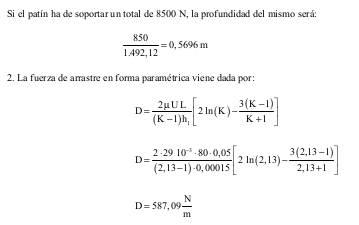
\includegraphics[scale=0.5]{Section_Files/S2-imagenes-Jhon/Book-ProbResuelts/P40-E04.png}
\end{figure}
Continúa...\\
{\tiny Mecánica de fluidos - Problemas resueltos por Josep Bergada Graño, pág. 150}
\end{frame}

\begin{frame}{PROBLEMAS RESUELTOS: Flujo con viscosidad dominante - 15/20}
\justifying
\begin{figure}[H]
\centering
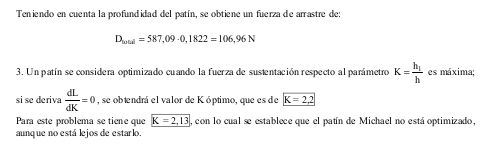
\includegraphics[scale=0.5]{Section_Files/S2-imagenes-Jhon/Book-ProbResuelts/P40-E05.png}
\end{figure}
{\tiny Mecánica de fluidos - Problemas resueltos por Josep Bergada Graño, pág. 150}
\end{frame}
		

%********************


\appendix
\section{Referencias}

\begin{frame}{Referencias}
\begin{thebibliography}{8}

\beamertemplatebookbibitems
\bibitem{Author19901}
Fundamentos y Aplicaciones de Mecánica de Fluidos.
\newblock{\em Yunus Cengel y John Cimbala}.
\newblock{Editorial McGraw-Hill (2006)}

\bibitem{Author00}
Mecánica de Fluidos - Problemas resueltos.
\newblock{\em Josep M. Bergadà Graño}.
\newblock{Editorial de la Universidad Politècnica de Catalunya (2006)}

\bibitem{Author01}
Biofluid Mechanics Applications.
\newblock{\em Ali Ostadfar}.
\newblock{Editorial Elsevier (2016)}

\bibitem{Author02}
Biofluid Mechanics
\newblock{\em David A. Rubenstein}.
\newblock{Editorial Elservier (2015)}

\end{thebibliography}
\end{frame}

\begin{frame}{Referencias}
\begin{thebibliography}{8}
\beamertemplatebookbibitems

\bibitem{Author03}
Introducción a la Dinámica de Fluidos.
\newblock{\em Yuri N. Skiba}.
\newblock{Editorial de la Universidad Nacional Autónoma de México (2008)}

\bibitem{Author04}
Applied Biofluid Mechanics.
\newblock{\em Lee Waite and Jerry Fine}.
\newblock{Editorial Mc Graw Hill (2007)}

\end{thebibliography}
\end{frame}

\end{document}